

% Gradient Info
  
\tikzset {_oo0z95nez/.code = {\pgfsetadditionalshadetransform{ \pgftransformshift{\pgfpoint{0 bp } { -1.5 bp }  }  \pgftransformrotate{-90 }  \pgftransformscale{2 }  }}}
\pgfdeclarehorizontalshading{_7ukztbkc5}{150bp}{rgb(0bp)=(1,1,1);
rgb(37.5bp)=(1,1,1);
rgb(62.5bp)=(0,0,0);
rgb(100bp)=(0,0,0)}
\tikzset{_fd5st3tr3/.code = {\pgfsetadditionalshadetransform{\pgftransformshift{\pgfpoint{0 bp } { -1.5 bp }  }  \pgftransformrotate{-90 }  \pgftransformscale{2 } }}}
\pgfdeclarehorizontalshading{_j0lyu8nds} {150bp} {color(0bp)=(transparent!0);
color(37.5bp)=(transparent!0);
color(62.5bp)=(transparent!10);
color(100bp)=(transparent!10) } 
\pgfdeclarefading{_l2sq6wasg}{\tikz \fill[shading=_j0lyu8nds,_fd5st3tr3] (0,0) rectangle (50bp,50bp); } 

% Gradient Info
  
\tikzset {_vl71yme9t/.code = {\pgfsetadditionalshadetransform{ \pgftransformshift{\pgfpoint{0 bp } { 0 bp }  }  \pgftransformscale{1 }  }}}
\pgfdeclareradialshading{_vlzwsksb4}{\pgfpoint{0bp}{0bp}}{rgb(0bp)=(1,1,1);
rgb(0bp)=(1,1,1);
rgb(25bp)=(0.96,0.65,0.14);
rgb(400bp)=(0.96,0.65,0.14)}
\tikzset{every picture/.style={line width=0.75pt}} %set default line width to 0.75pt        

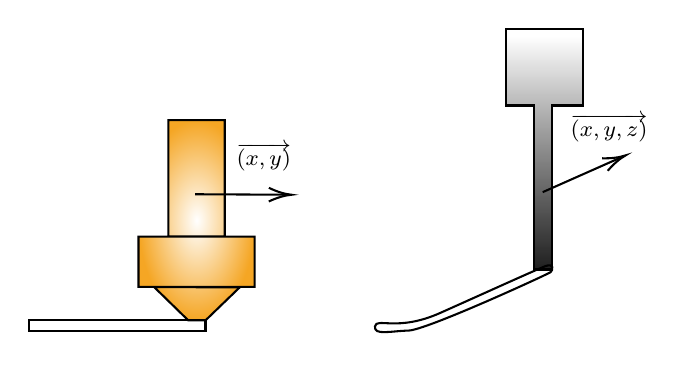
\begin{tikzpicture}[x=0.75pt,y=0.75pt,yscale=-1,xscale=1]
%uncomment if require: \path (0,300); %set diagram left start at 0, and has height of 300

%Shape: Path Data [id:dp6219748067424139] 
\path  [shading=_7ukztbkc5,_oo0z95nez,path fading= _l2sq6wasg ,fading transform={xshift=2}] (349.5,135.25) -- (341,135.25) -- (341,56.25) -- (327.5,56.25) -- (327.5,19.25) -- (364.5,19.25) -- (364.5,56.25) -- (349.5,56.25) -- (349.5,135.25) -- cycle ; % for fading 
 \draw   (349.5,135.25) -- (341,135.25) -- (341,56.25) -- (327.5,56.25) -- (327.5,19.25) -- (364.5,19.25) -- (364.5,56.25) -- (349.5,56.25) -- (349.5,135.25) -- cycle ; % for border 

%Shape: Path Data [id:dp1918091195313667] 
\path  [shading=_vlzwsksb4,_vl71yme9t] (182.55,159.77) -- (174.21,159.74) -- (157.81,143.73) -- (199.03,143.86) -- (182.55,159.77) -- cycle (206.25,143.67) -- (150.25,143.67) -- (150.25,119.45) -- (206.25,119.45) -- (206.25,143.67) -- cycle (191.82,63.25) -- (191.82,119.27) -- (164.68,119.27) -- (164.68,63.25) -- (191.82,63.25) -- cycle ; % for fading 
 \draw   (182.55,159.77) -- (174.21,159.74) -- (157.81,143.73) -- (199.03,143.86) -- (182.55,159.77) -- cycle (206.25,143.67) -- (150.25,143.67) -- (150.25,119.45) -- (206.25,119.45) -- (206.25,143.67) -- cycle (191.82,63.25) -- (191.82,119.27) -- (164.68,119.27) -- (164.68,63.25) -- (191.82,63.25) -- cycle ; % for border 

%Shape: Regular Polygon [id:dp2406449410310607] 
\draw   (264.2,162.67) .. controls (264.78,158.17) and (274.8,165.47) .. (295.58,156.21) .. controls (316.35,146.94) and (341.69,135.43) .. (346.21,133.68) .. controls (350.73,131.94) and (349.89,135.66) .. (348.81,136.54) .. controls (347.74,137.42) and (288.95,164.48) .. (280.3,164.69) .. controls (271.66,164.9) and (263.61,167.16) .. (264.2,162.67) -- cycle ;
%Straight Lines [id:da5529504218441703] 
\draw    (177.5,99) -- (222,99.24) ;
\draw [shift={(224,99.25)}, rotate = 180.31] [color={rgb, 255:red, 0; green, 0; blue, 0 }  ][line width=0.75]    (10.93,-3.29) .. controls (6.95,-1.4) and (3.31,-0.3) .. (0,0) .. controls (3.31,0.3) and (6.95,1.4) .. (10.93,3.29)   ;
%Straight Lines [id:da9164514520029656] 
\draw    (345,98) -- (383.17,81.06) ;
\draw [shift={(385,80.25)}, rotate = 156.07] [color={rgb, 255:red, 0; green, 0; blue, 0 }  ][line width=0.75]    (10.93,-3.29) .. controls (6.95,-1.4) and (3.31,-0.3) .. (0,0) .. controls (3.31,0.3) and (6.95,1.4) .. (10.93,3.29)   ;
%Shape: Rectangle [id:dp6644461740443299] 
\draw   (97.37,159.77) -- (182.55,159.77) -- (182.55,164.78) -- (97.37,164.78) -- cycle ;

% Text Node
\draw (196,73) node [anchor=north west][inner sep=0.75pt]  [font=\footnotesize] [align=left] {$\displaystyle \overrightarrow{( x,y)}$};
% Text Node
\draw (357,59) node [anchor=north west][inner sep=0.75pt]  [font=\footnotesize] [align=left] {$\displaystyle \overrightarrow{( x,y,z)}$};


\end{tikzpicture}
